\section{Results}

\subsection{Model quality in the map and financial features}

\begin{table}[htbp]
\centering\caption{UMAP and t-SNE fitted through the same pipeline. Scores describe the representative seed-42 partition, which includes all 41 instruments; S is silhouette and DB Davies-Bouldin; seed ARI is the mean of ten pairwise comparisons; sector ARI compares the partition with the recorded sector labels.}\label{tab:method_quality}
\footnotesize
\begin{tabularx}{\linewidth}{@{}>{\raggedright\arraybackslash}X l r r r r r r r@{}}
\toprule
Date & Method & Feature S & Feature DB & Map S & Map DB & Singletons & Seed ARI & Sector ARI \\
\midrule
June 2025 & UMAP & 0.151 & 1.153 & 0.685 & 0.385 & 0 & 0.846 & 0.152 \\
 & t-SNE & 0.195 & 1.307 & 0.532 & 0.561 & 0 & 0.658 & 0.276 \\
December 2025 & UMAP & 0.124 & 1.049 & 0.638 & 0.268 & 2 & 0.892 & 0.318 \\
 & t-SNE & 0.240 & 1.094 & 0.589 & 0.494 & 0 & 0.925 & 0.333 \\
June 2026 & UMAP & 0.267 & 1.059 & 0.721 & 0.355 & 0 & 0.738 & 0.472 \\
 & t-SNE & 0.255 & 1.016 & 0.656 & 0.390 & 0 & 0.894 & 0.417 \\
\bottomrule
\end{tabularx}
\end{table}

The clusters were more clearly separated in the UMAP maps than in the original financial features (Table~\ref{tab:method_quality}). Map Silhouette Scores were 0.685, 0.638 and 0.721 across the three dates. Financial-feature scores were 0.151, 0.124 and 0.267. UMAP had higher map scores than t-SNE at every date, but t-SNE had higher financial-feature scores in June and December 2025. Map separation therefore needs to be read alongside similarity in the financial data. UMAP group sizes ranged from two to nine, one to eight and two to eight instruments, respectively. Only December contained single-member clusters.

December 2025 gave the most consistent UMAP grouping across the tested seeds, despite containing two single-member clusters. Mean seed ARI was 0.846, 0.892 and 0.738 across the three dates. Pairwise scores ranged from 0.71 to 1.00 in June 2025, 0.81 to 0.96 in December 2025 and 0.60 to 0.90 in June 2026. Group size and seed agreement therefore describe different aspects of the result. Because these pairs share fitted models, their spread is not a confidence interval for changes over time.

No model combination performed best on every measure (Table~\ref{tab:model_comparison}). The table compares PCA, t-SNE and default UMAP with hierarchical clustering, K-Means and DBSCAN, alongside the study model. Default UMAP uses ten neighbours and a minimum distance of 0.1. Hierarchical clustering and K-Means use eight groups. DBSCAN chooses its own group count and excludes noise observations from scoring. Its sometimes higher scores concern two to five groups and, for PCA, fewer than all instruments. Coverage therefore matters when comparing these scores.

\begin{table}[htbp]
\centering\caption{Complete comparison of dimensionality-reduction and clustering combinations at the representative seed. Map scores use the reduced representation and feature scores the eight scaled financial features. Combinations without a stated group count use eight groups and assign all 41 instruments; DBSCAN chooses its own number of groups, and its scores exclude noise observations.}\label{tab:model_comparison}
\footnotesize
\begin{tabularx}{\linewidth}{@{}>{\raggedright\arraybackslash}X l l r r r r r r@{}}
\toprule
Reduction & Clustering & Date & Groups & Coverage & Map S & Map DB & Feature S & Feature DB \\
\midrule
UMAP (study model) & Hierarchical & Jun 2025 & 8 & 100\% & 0.685 & 0.385 & 0.151 & 1.153 \\
 &  & Dec 2025 & 8 & 100\% & 0.638 & 0.268 & 0.124 & 1.049 \\
 &  & Jun 2026 & 8 & 100\% & 0.721 & 0.355 & 0.267 & 1.059 \\
\addlinespace[2pt]
t-SNE & Hierarchical & Jun 2025 & 8 & 100\% & 0.532 & 0.561 & 0.195 & 1.307 \\
 &  & Dec 2025 & 8 & 100\% & 0.589 & 0.494 & 0.240 & 1.094 \\
 &  & Jun 2026 & 8 & 100\% & 0.656 & 0.390 & 0.255 & 1.016 \\
\addlinespace[2pt]
t-SNE & K-Means & Jun 2025 & 8 & 100\% & 0.522 & 0.590 & 0.201 & 1.300 \\
 &  & Dec 2025 & 8 & 100\% & 0.637 & 0.418 & 0.245 & 1.070 \\
 &  & Jun 2026 & 8 & 100\% & 0.596 & 0.612 & 0.247 & 1.140 \\
\addlinespace[2pt]
t-SNE & DBSCAN & Jun 2025 & 5 & 100\% & 0.469 & 0.561 & 0.243 & 1.154 \\
 &  & Dec 2025 & 4 & 100\% & 0.494 & 0.505 & 0.327 & 1.052 \\
 &  & Jun 2026 & 5 & 100\% & 0.680 & 0.447 & 0.279 & 1.173 \\
\addlinespace[2pt]
UMAP (default) & Hierarchical & Jun 2025 & 8 & 100\% & 0.467 & 0.601 & 0.142 & 1.151 \\
 &  & Dec 2025 & 8 & 100\% & 0.547 & 0.528 & 0.240 & 1.043 \\
 &  & Jun 2026 & 8 & 100\% & 0.507 & 0.681 & 0.266 & 1.157 \\
\addlinespace[2pt]
UMAP (default) & K-Means & Jun 2025 & 8 & 100\% & 0.441 & 0.658 & 0.152 & 1.260 \\
 &  & Dec 2025 & 8 & 100\% & 0.547 & 0.528 & 0.240 & 1.043 \\
 &  & Jun 2026 & 8 & 100\% & 0.519 & 0.641 & 0.256 & 1.172 \\
\addlinespace[2pt]
UMAP (default) & DBSCAN & Jun 2025 & 3 & 100\% & 0.278 & 0.684 & -0.048 & 1.484 \\
 &  & Dec 2025 & 2 & 100\% & 0.773 & 0.235 & 0.588 & 0.584 \\
 &  & Jun 2026 & 2 & 100\% & 0.701 & 0.313 & 0.430 & 0.826 \\
\addlinespace[2pt]
PCA & Hierarchical & Jun 2025 & 8 & 100\% & 0.375 & 0.541 & 0.206 & 1.051 \\
 &  & Dec 2025 & 8 & 100\% & 0.436 & 0.457 & 0.230 & 0.878 \\
 &  & Jun 2026 & 8 & 100\% & 0.458 & 0.505 & 0.229 & 1.103 \\
\addlinespace[2pt]
PCA & K-Means & Jun 2025 & 8 & 100\% & 0.369 & 0.748 & 0.135 & 1.422 \\
 &  & Dec 2025 & 8 & 100\% & 0.398 & 0.647 & 0.168 & 1.163 \\
 &  & Jun 2026 & 8 & 100\% & 0.429 & 0.638 & 0.138 & 1.612 \\
\addlinespace[2pt]
PCA & DBSCAN & Jun 2025 & 2 & 76\% & 0.593 & 0.402 & 0.458 & 0.586 \\
 &  & Dec 2025 & 2 & 78\% & 0.586 & 0.453 & 0.412 & 0.837 \\
 &  & Jun 2026 & 4 & 90\% & 0.541 & 0.484 & 0.393 & 1.077 \\
\bottomrule
\end{tabularx}

\end{table}

Section~\ref{sec:method_comparison} examines whether UMAP and t-SNE identify the same persistent groups and membership changes.

% BEGIN CLUSTER MAPS AND TREES
\FloatBarrier
\subsection{Cluster maps and hierarchical structure}

The three maps show eight groups at each date, with their members and financial-feature and map quality scores (Figures~\ref{fig:clusters_tree_2025-06-30}--\ref{fig:clusters_tree_2026-06-30}). Each includes all 41 instruments from the representative seed-42 fit. An asterisk marks an imputed input. Cluster numbers and colours use the matched labels, allowing groups to be followed into the membership histories and financial profiles. Gaps in numbering indicate labels absent at that date. Positions cannot be compared directly between maps because UMAP was fitted independently at each date.

Each dendrogram shows how the hierarchy joins instruments and groups in the corresponding UMAP map. The model uses average linkage and Manhattan distance. Leaves identify tickers and recorded sectors. Branch heights measure linkage distance, not statistical significance. Branch colours are plotting conventions and do not define the eight clusters.

\begin{figure}[htbp]
\centering
\clusterpair{2025-06-30}
\caption{30 June 2025: UMAP cluster map (left) and dendrogram (right) for the representative seed-42 partition. All 41 instruments are included. Cluster numbers are aligned across dates; an asterisk marks an imputed input. Tree leaves show tickers and recorded sectors; branch colours are independent of cluster colours.}\label{fig:clusters_tree_2025-06-30}
\end{figure}

\begin{figure}[htbp]
\centering
\clusterpair{2025-12-31}
\caption{31 December 2025: UMAP cluster map and dendrogram, as in Figure~\ref{fig:clusters_tree_2025-06-30}.}\label{fig:clusters_tree_2025-12-31}
\end{figure}

\begin{figure}[htbp]
\centering
\clusterpair{2026-06-30}
\caption{30 June 2026: UMAP cluster map and dendrogram, as in Figure~\ref{fig:clusters_tree_2025-06-30}.}\label{fig:clusters_tree_2026-06-30}
\end{figure}

\FloatBarrier
% END CLUSTER MAPS AND TREES

\subsection{How companies move between clusters over time}

\begin{table}[htbp]
\centering\caption{Temporal comparison among the 40 continuing instruments in each adjacent pair. Entries and exits are excluded from changed and unchanged counts.}\label{tab:6}
\footnotesize
\begin{tabularx}{\linewidth}{@{}>{\hsize=1.750\hsize\linewidth=\hsize\raggedright\arraybackslash}X >{\hsize=0.700\hsize\linewidth=\hsize\raggedright\arraybackslash}X >{\hsize=0.910\hsize\linewidth=\hsize\raggedright\arraybackslash}X >{\hsize=1.050\hsize\linewidth=\hsize\raggedright\arraybackslash}X >{\hsize=1.050\hsize\linewidth=\hsize\raggedright\arraybackslash}X >{\hsize=0.770\hsize\linewidth=\hsize\raggedright\arraybackslash}X >{\hsize=0.770\hsize\linewidth=\hsize\raggedright\arraybackslash}X@{}}
\toprule
Period & Continue & Entry / exit & Changed & Unchanged & ARI & NMI \\
\midrule
Jun-Dec 2025 & 40 & 1 / 1 & 15 (37.5\%) & 25 (62.5\%) & 0.377 & 0.646 \\
Dec 2025-Jun 2026 & 40 & 1 / 1 & 11 (27.5\%) & 29 (72.5\%) & 0.590 & 0.751 \\
\bottomrule
\end{tabularx}
\end{table}


Fewer continuing instruments changed groups in the second interval than in the first (Table~\ref{tab:6}). Fifteen of 40 changed between June and December 2025, compared with 11 between December 2025 and June 2026. Temporal ARI increased from 0.377 to 0.590, also indicating greater agreement in the second comparison. Among the 39 instruments observed throughout, 19 retained their matched group and 20 changed at least once. Five changed twice and 15 changed once, accounting for 25 switch events. Mondi contributes the remaining first-period switch before leaving the index. These two comparisons do not establish a statistically significant trend.


Figure~\ref{fig:flows} shows all 39 complete membership histories. Absa, Discovery, Old Mutual, Remgro and Reinet changed groups in both periods. The examples below contrast persistent peer groups with fragmented groups and individual transitions. Index entries and exits are excluded only from the complete three-date diagram.



\begin{figure}[htbp]
\centering
\diagram{flows}
\caption{Cluster membership across the three decision dates for the 39 continuously observed instruments. Bold tickers change aligned group at least once. APN, MNP, GLN and PAN are excluded only from this complete-history view. Colours and labels identify aligned groups, not sectors; vertical positions are layout.}\label{fig:flows}
\end{figure}


\subsection{Interpretation of cluster changes}\label{sec:cluster_changes}


\begin{figure}[htbp]
\centering
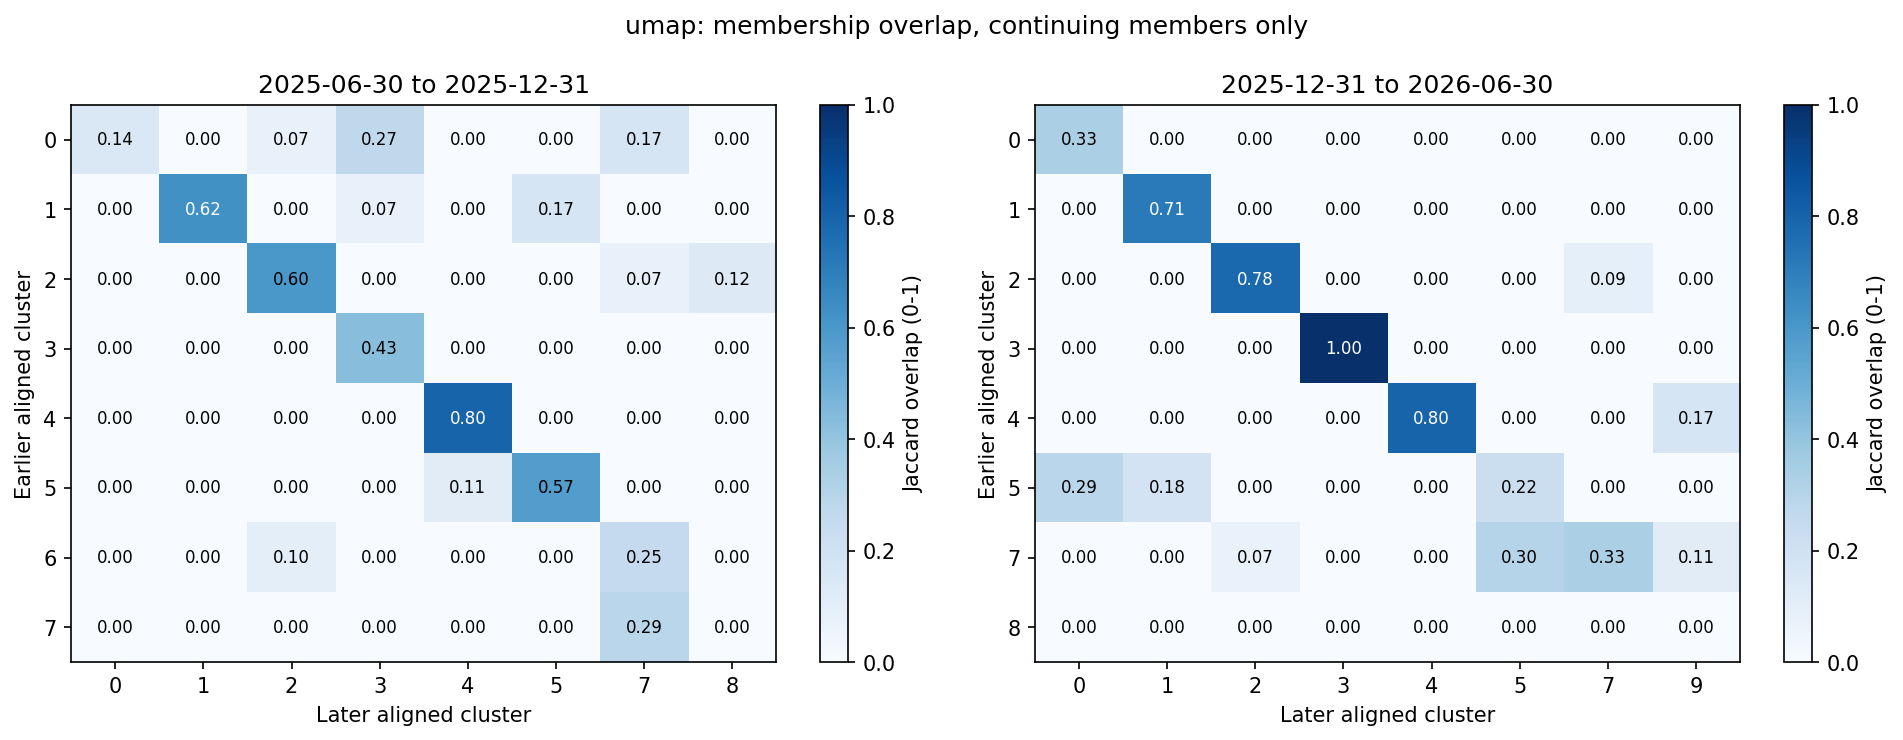
\includegraphics[width=\linewidth]{figures/python/jaccard.png}
\caption{Jaccard overlap among the 40 continuing members in each adjacent comparison. Each cell uses the common eligible universe for that period. Numeric values are given explicitly; a zero denotes no shared continuing member.}\label{fig:jaccard}
\end{figure}


Keeping a cluster label does not mean keeping all its members. Figure~\ref{fig:jaccard} shows the overlaps used for matching. Five of the eight continuing members of June 2025 group 1 remain in December group 1, giving Jaccard similarity 0.625. The earlier members were Absa (ABG), Growthpoint (GRT), Investec Limited (INL), Investec plc (INP), Nedbank (NED), NEPI Rockcastle (NRP), Old Mutual (OMU) and Valterra Platinum (VAL). Some other matches have lower overlap. Matching maximises total similarity across all group pairs, so individual matches must also be checked against their members.


June 2025 group 0 fragmented into four destinations by December (Figure~\ref{fig:flows}). AngloGold Ashanti (ANG), Gold Fields (GFI) and Harmony (HAR) moved to group 3. Discovery (DSY) and MTN moved to group 7, and Pepkor (PPH) moved to group 2. Only OUTsurance (OUT) retained group 0. June group 6 also dispersed: Clicks (CLS) joined group 2, while Remgro (REM) and Reinet (RNI) joined group 7. Its label was retired. The weaker overlaps in Figure~\ref{fig:jaccard} help identify this fragmentation, which a retained label alone cannot describe.

Absa and Old Mutual returned to an earlier matched group, following $1\rightarrow5\rightarrow1$. Absa also changed groups under t-SNE, whereas Old Mutual did not (Section~\ref{sec:method_comparison}). In the first interval, Absa's dividend yield fell by 0.196 June 2025 reference-scaled units, while Old Mutual's one-year return rose by 0.175. In the second interval, beta fell by 0.137 and 0.186 units, respectively. Their June 2026 destination had relatively high dividend and earnings yields (Figure~\ref{fig:profiles}(c)). Returning to earlier peers therefore describes renewed financial similarity, not a reversal of every financial variable.

Naspers (NPN) and Prosus (PRX) joined group 9 in June 2026, having previously occupied groups 7 and 4. Their one-year returns fell by 0.468 and 0.527 reference-scaled units between December and June. The destination group had relatively high market capitalisation and low return and dividend yield (Figure~\ref{fig:profiles}(c)). Sasol (SOL) instead moved from group 2 to group 7. Its beta fell by 0.642 and one-year return rose by 0.627 units. Reinet followed $6\rightarrow7\rightarrow2$, although imputed fundamentals limit its interpretation. These changes use saved instrument records and the fixed June 2025 scale. They describe measured changes, not causal effects or SHAP attributions. No single feature is assumed to determine membership.

The surrogate uses different features to support different destination labels (Table~\ref{tab:move_shap}). Return supports the December precious-metals assignments, alongside measured return increases for AngloGold Ashanti, Gold Fields and Valterra. Both mapping methods recover the December group, but the switches of AngloGold Ashanti and Gold Fields into it occur only under UMAP. In June, dividend yield and earnings yield support group 1 for Absa and Old Mutual, although beta is among their larger measured changes. Return, earnings yield and dividend yield support group 9 for Naspers and Prosus. Return gives the strongest support to Sasol's group-7 assignment. A feature that changes substantially is therefore not necessarily the feature the surrogate uses most strongly to reproduce a label. Each grouped table row contains identical individual contributions before rounding; none is an average or a representative selected equity.

\begin{table}[htbp]
\centering
\caption{Selected positive Tree SHAP contributions to destination-cluster raw margins. Each value applies individually to every equity in its row: contributions are identical before rounding, not averages. Values from the fully fitted date-specific surrogate are raw margins, not probabilities or changes in financial units. Destination groups use aligned labels.}\label{tab:move_shap}
\footnotesize
\begin{tabularx}{\linewidth}{@{}>{\raggedright\arraybackslash}p{2.0cm}>{\raggedright\arraybackslash}p{2.0cm}p{1.1cm}X@{}}
\toprule
Date & Instruments & Group & Feature contributions \\
\midrule
Dec 2025 & ANG, GFI, VAL & 3 & Return $+2.933$ \\
Jun 2026 & ABG, OMU & 1 & Dividend yield $+2.863$; earnings yield $+0.054$ \\
Jun 2026 & NPN, PRX & 9 & Return $+1.435$; earnings yield $+0.685$; dividend yield $+0.468$ \\
Jun 2026 & SOL & 7 & Return $+2.016$; dividend yield $+0.686$; volatility $+0.225$ \\
\bottomrule
\end{tabularx}
\end{table}
\FloatBarrier

Positive SHAP values increase the destination class's raw margin relative to its expected margin. These baselines differ by date and class, so contributions are not a common financial scale across groups or dates. We could not test December fidelity on held-out instruments because of single-member clusters. June 2026 fidelity was 0.707 (Section~\ref{sec:surrogate}). The December attributions therefore describe the fitted classifier without a held-out check, and the June attributions supplement the direct financial profiles. They explain reproduced labels rather than causes of financial change.

\subsection{Financial feature profiles}

The heatmaps show how each group's financial characteristics differ from the same-date population median (Figure~\ref{fig:profiles}). Values use the fixed June 2025 scale. Positive values are relatively high and negative values relatively low. All 41 instruments are included at each date. Matched group labels allow the three profiles to be read alongside the membership histories.

\begin{figure}[htbp]
\centering
\profilepanel{(a) 30 June 2025}{profile0}\par\medskip
\profilepanel{(b) 31 December 2025}{profile1}\par\medskip
\profilepanel{(c) 30 June 2026}{profile2}
\caption{Aligned-cluster median deviations from the same-date median, in June 2025 MinMax units. Counts include all 41 date-specific instruments. All panels use one colour scale from $-1.5$ (blue) to $+1.5$ (red), with zero at the same-date median; gaps in cluster numbers reflect retired identifiers.}\label{fig:profiles}
\end{figure}

\FloatBarrier

Precious-metals companies maintained a core group while attracting additional members. Impala Platinum, Northam Platinum and Sibanye-Stillwater formed group 3 in June 2025 and remained together at all three dates. AngloGold Ashanti, Gold Fields, Harmony and Valterra joined by December, increasing membership from three to seven. Pan African Resources entered the index and joined in June 2026, bringing membership to eight. The t-SNE comparator grouped all seven December members together in every seed. In its representative June 2025 fit, AngloGold Ashanti, Gold Fields and Harmony already shared the platinum group. That earlier association appeared in only two of five seeds. Valterra was therefore the only switch into the group under the representative t-SNE fit. The maps and Figure~\ref{fig:flows} show these membership differences.

High volatility, beta and return characterised the initial three-member precious-metals group (Figure~\ref{fig:profiles}(a)). In December, its median return was 1.45 reference-scaled units above the population median, alongside elevated volatility and beta (panel b). AngloGold Ashanti, Gold Fields and Valterra recorded return increases of 1.342, 1.143 and 0.940 reference-scaled units over that interval. These changes are consistent with the destination group's return profile. High volatility and beta remained prominent in June 2026 (panel c). The figures show a persistent peer core with changing membership. They do not establish a commodity-price cause or predict future returns.

Anheuser-Busch InBev (ANH), BHP (BHG) and Richemont (CFR) formed a second persistent core in group 4. Prosus joined them at the first two dates and left by June 2026. British American Tobacco joined in December. The group consistently had relatively high log market capitalisation and low JSE share turnover (Figure~\ref{fig:profiles}). June 2026 deviations were approximately $+0.65$ and $-0.64$ reference-scaled units, respectively. These cross-sector peers share size and local trading characteristics. Low JSE turnover does not establish low global liquidity because internationally listed firms also trade elsewhere.

\subsection{Agreement with sector labels}

The clusters became more closely aligned with recorded sectors over the three dates (Table~\ref{tab:sector}). ARI rose from 0.152 to 0.318 and 0.472, while Normalised Mutual Information rose from 0.447 to 0.719. We describe an instrument as sector-divergent when its sector differs from the most common sector among its cluster peers. We do not classify single-member clusters or clusters with tied majorities. The number of divergent instruments fell from 17 to 9 and then 5. Much of this change reflects the precious-metals group, whose June 2026 members all belong to basic materials.

\begin{table}[htbp]
\centering\caption{Agreement between the UMAP clusters and the recorded sector labels, and the sector-divergent instruments at each date.}\label{tab:sector}
\footnotesize
\begin{tabularx}{\linewidth}{@{}l r r r >{\raggedright\arraybackslash}X@{}}
\toprule
Date & Sector ARI & Sector NMI & Divergent & Instruments whose sector differs from their cluster majority \\
\midrule
Jun 2025 & 0.152 & 0.447 & 17 & AGL, APN, BHG, BTI, BVT, CLS, CPI, DSY, MNP, MTN, NPN, OUT, PPH, PRX, SOL, VAL, VOD \\
Dec 2025 & 0.318 & 0.585 & 9 & AGL, BHG, BVT, GLN, MTN, NPN, PRX, SOL, VOD \\
Jun 2026 & 0.472 & 0.719 & 5 & BHG, BVT, MTN, RNI, VOD \\
\bottomrule
\end{tabularx}

\end{table}

BHP, Bidvest, MTN and Vodacom differed from their cluster peers' sectors at all three dates. BHP grouped with consumer-goods and technology companies rather than other basic-materials companies. Bidvest, an industrial company, grouped with consumer-services retailers. The telecommunications companies MTN and Vodacom never shared a cluster. MTN grouped with basic-materials and financial companies, while Vodacom grouped with financial companies. These cases show where measured financial characteristics repeatedly place a company alongside peers from other sectors.

\subsection{Economic validation through forward co-movement}\label{sec:comovement}

Cluster peers did not have more similar subsequent returns than sector peers. Sector peers moved together more strongly in both evaluation periods (Table~\ref{tab:comovement}). For raw returns, $\Delta\rho$ was $-0.129$ after June 2025 and $-0.069$ after December 2025. Both 95\% intervals excluded zero, rejecting the primary hypothesis. Market adjustment lowered every correlation but left similar differences of $-0.112$ and $-0.068$. The result held for every UMAP seed and for t-SNE. Clusters nevertheless co-moved more strongly than random groups of the same sizes, with permutation $p<0.001$ at both dates.

Giving every company equal weight did not change the conclusion. We first averaged each instrument's cluster-minus-sector contrast within its company and then across companies, rather than averaging over pairs. The differences were $-0.117$ and $-0.083$, compared with pair-averaged estimates of $-0.129$ and $-0.069$. The difference remained negative when companies were weighted equally. This check concerns the primary comparison, not the follow-up analysis below.

\begin{table}[htbp]
\centering\caption{Mean forward correlation of daily returns between peers over the six months after each formation date. $\Delta\rho$ is cluster peers minus sector peers; the interval is from a ten-day block bootstrap. Market-adjusted returns are residuals from a regression on the Top 40 Index.}\label{tab:comovement}
\footnotesize
\begin{tabularx}{\linewidth}{@{}l >{\raggedright\arraybackslash}X r r r r r@{}}
\toprule
Formed & Returns & Cluster peers & Sector peers & All pairs & $\Delta\rho$ & 95\% interval \\
\midrule
Jun 2025 & Raw & 0.215 & 0.344 & 0.140 & -0.129 & [-0.171, -0.096] \\
Jun 2025 & Market-adjusted & 0.131 & 0.244 & 0.031 & -0.112 & [-0.159, -0.077] \\
Dec 2025 & Raw & 0.381 & 0.449 & 0.252 & -0.069 & [-0.100, -0.040] \\
Dec 2025 & Market-adjusted & 0.209 & 0.277 & 0.040 & -0.068 & [-0.112, -0.032] \\
\bottomrule
\end{tabularx}

\end{table}

In an exploratory analysis, companies in the same sector and cluster had more similar subsequent returns than companies in the same sector but different clusters (Table~\ref{tab:comovement_pairs}). This follow-up analysis was developed after seeing the primary result. Raw correlations were 0.391 against 0.329 after June 2025, and 0.552 against 0.396 after December 2025.

A regression accounting for shared sector membership also gave a positive cluster coefficient at both dates, for raw and market-adjusted returns. Under global reassignment of cluster labels, permutation $p$ values ranged from 0.001 to 0.019. These p-values concern the additive coefficient under a global exchangeability null, not a within-sector randomisation null. The observed pair means suggest that the additional information comes mainly from within sectors. Pairs sharing a cluster across sectors co-moved little more than unrelated pairs. Their market-adjusted correlations were 0.007 and 0.021, compared with $-0.034$ and $-0.037$ for unrelated pairs. For raw returns after December 2025, they co-moved less than unrelated pairs.

\begin{table}[htbp]
\centering\caption{Mean forward correlation by type of pair, with the number of pairs after June and December 2025. The cluster coefficient is from a regression of pairwise correlation on shared-sector and shared-cluster indicators. Permutation $p$-values use 5,000 random reassignments of cluster labels across instruments, preserving cluster sizes.}\label{tab:comovement_pairs}
\footnotesize
\begin{tabularx}{\linewidth}{@{}>{\raggedright\arraybackslash}X r r r r@{}}
\toprule
Pairs & Jun 2025 raw & Jun 2025 adj. & Dec 2025 raw & Dec 2025 adj. \\
\midrule
Same sector, same cluster (41; 65 pairs) & 0.391 & 0.331 & 0.552 & 0.342 \\
Same sector, other cluster (138; 125 pairs) & 0.329 & 0.218 & 0.396 & 0.243 \\
Other sector, same cluster (66; 46 pairs) & 0.105 & 0.007 & 0.139 & 0.021 \\
Other sector, other cluster (574; 583 pairs) & 0.079 & -0.034 & 0.195 & -0.037 \\
\midrule
Cluster coefficient & 0.038 & 0.066 & 0.050 & 0.078 \\
Permutation $p$ & 0.019 & 0.003 & 0.009 & 0.001 \\
\bottomrule
\end{tabularx}

\end{table}

The sector-restricted sensitivity retained positive within-sector differences but gave more qualified statistical evidence. Table~\ref{tab:sector_conditioned_sensitivity} gives all eight direct contrasts, intervals and restricted-permutation p-values. For UMAP raw returns, the differences were 0.062 after June 2025 (conditional bootstrap 95\% interval 0.015--0.091) and 0.157 after December (0.098--0.203). Their restricted-permutation p-values were 0.029 and 0.0004; Holm-adjusted values across the 16 sensitivity tests were 0.059 and 0.006. Market-adjusted contrasts were also positive, with adjusted p-values of 0.036 and 0.006. For t-SNE, all four direct contrasts remained positive with adjusted p-values below 0.05. The additive-coefficient test was not uniformly below that threshold either: raw UMAP December had adjusted $p=0.059$. The bootstrap intervals describe uncertainty in the realised return panel, while the permutation tests compare label allocations under their stated null. These distinct checks support a qualified exploratory interpretation, not uniform statistical support across specifications.


The contrast between individual groups reinforces the difference between financial similarity and return similarity. Precious-metals peers co-moved strongly, with mean raw correlations of 0.82 and 0.81. The large-capitalisation, low-turnover group co-moved weakly, at 0.11 and 0.05. Similar size and JSE trading activity therefore did not imply similar subsequent returns. The t-SNE comparator performed at least as well as UMAP. After June 2025, its cluster coefficient was larger, at 0.089 against 0.038 for raw returns; after December, the coefficients were similar.

\subsection{Sensitivity to the choice of representation}\label{sec:method_comparison}

Changing from UMAP to t-SNE affected model scores and some membership changes (Table~\ref{tab:method_quality}). The t-SNE financial-feature Silhouette Score was higher in June and December 2025. It contained no single-member clusters and had greater seed agreement in December 2025 and June 2026. It recorded 9 switches in each interval, compared with 15 and 11 under UMAP. The two methods' groupings nevertheless agreed substantially: their ARI was 0.635, 0.800 and 0.923 across the three dates. Table~\ref{tab:method_groups} examines whether they also recover the same selected financial peer groups across seeds.

\begin{table}[htbp]
\centering\caption{Number of the five seeds in which every listed equity is assigned to the same cluster.}\label{tab:method_groups}
\footnotesize
\begin{tabularx}{\linewidth}{@{}>{\raggedright\arraybackslash}X ccc ccc@{}}
\toprule
 & \multicolumn{3}{c}{UMAP} & \multicolumn{3}{c}{t-SNE} \\
\cmidrule(lr){2-4}\cmidrule(l){5-7}
Group & Jun 2025 & Dec 2025 & Jun 2026 & Jun 2025 & Dec 2025 & Jun 2026 \\
\midrule
Platinum core: IMP, NPH, SSW & 5 & 5 & 4 & 5 & 5 & 5 \\
Platinum core with ANG, GFI, HAR & 0 & 5 & 4 & 2 & 5 & 5 \\
Platinum core with ANG, GFI, HAR, VAL & 0 & 5 & 4 & 0 & 5 & 5 \\
Scale core: ANH, BHG, CFR & 5 & 5 & 5 & 5 & 5 & 5 \\
Naspers and Prosus & 1 & 0 & 5 & 2 & 0 & 5 \\
Absa and Old Mutual & 5 & 5 & 4 & 5 & 0 & 5 \\
\bottomrule
\end{tabularx}
\end{table}

Both methods produced similar main findings. They retained the platinum core and the large-capitalisation, low-turnover core throughout. Both placed the gold miners and Valterra with the precious-metals group in December 2025. Both joined Naspers and Prosus in June 2026 in every seed. The main difference concerned June 2025: t-SNE grouped the gold miners with the platinum core in two of five seeds, while UMAP never did. Absa and Old Mutual also separated in December under t-SNE but remained together under UMAP.

The two representations give the same stable or shifted classification for 28 of the 39 complete histories. Thirteen equities change group under both methods, and fifteen remain stable under both. Seven changes occur under UMAP only, and four under t-SNE only. Shared changes, including those of Sasol, Valterra, Naspers and Prosus, provide more robust candidates for analyst investigation. Method-specific changes, such as Old Mutual's under UMAP, remain informative but depend partly on the modelling choice.

UMAP remains useful for inspecting financial peer groups, but its clearer map separation does not establish greater investment relevance. The comparison recovers persistent groups and many membership changes under t-SNE. The forward test also finds that t-SNE performs at least as well (Section~\ref{sec:comovement}).

\subsection{Robustness and practical reading}

A fixed scale does not keep each feature's influence constant over time. In December 2025, one-year return accounted for 52.5\% of scaled variance, compared with 12.5\% under an even eight-variable allocation. The maximum scaled value was 2.847. Feature variance was less concentrated at the other dates. Dividend yield contributed the largest share in June 2025, at 19.8\%, and volatility in June 2026, at 22.1\%. Maximum scaled values were 1.000 and 1.244. Return's large December contribution matters because group changes can reflect both changing company characteristics and their relative influence after scaling.

Membership histories changed when the features changed. The untransformed ten-feature alternative (original10) agreed with the reference UMAP grouping at ARI 0.668, 0.607 and 0.590 across the three dates. Among the 39 continuously observed instruments, original10 gave 20 stable and 19 shifted histories. The corresponding counts were 16 and 23 for logsize10, 19 and 20 for invariant8, and 14 and 25 for market5. These alternatives represent size, liquidity and share-basis effects differently. Their switch counts show sensitivity to feature choices, rather than estimates of true economic change. Scores calculated in different feature spaces cannot be used as a single ranking of feature sets.

No cluster count performed best on every measure or at every date (Figure~\ref{fig:cluster_count}). We compared two to twelve groups. Financial-feature Silhouette Scores were highest at two groups in both 2025 observations and at seven in June 2026. Map Silhouette Scores were highest at nine, six and six groups. Eight groups is therefore a reference specification, not a uniquely optimal choice. Both the features and the number of groups influence the reported financial relationships.

\begin{figure}[htbp]
\centering
\diagram{cluster_count}
\caption{Cluster-count sensitivity from two to twelve groups. Blue lines show financial-feature scores and red lines embedding scores. Eight groups remain the reference specification.}\label{fig:cluster_count}
\end{figure}

\subsection{Surrogate interpretation and multivariate outliers}\label{sec:surrogate}

The surrogate reproduced all training labels, but agreement was weaker for held-out instruments. Out-of-fold fidelity was 43.9\% in June 2025 and 70.7\% in June 2026. The smallest group contained two instruments, limiting stratified cross-validation to two folds. We could not estimate December fidelity under this procedure because two clusters contained only one instrument. Direct financial profiles therefore provide the main explanation, with SHAP offering supplementary evidence about the features used to reproduce labels.

\begin{table}[htbp]
\centering\caption{Separate same-date Mahalanobis distance screen at nominal alpha 0.05. The reference value is 14.03 at each date ($n=41$, $p=8$). These are descriptive flags, not significant economic anomalies.}\label{tab:9}
\footnotesize
\begin{tabularx}{\linewidth}{@{}>{\hsize=0.720\hsize\linewidth=\hsize\raggedright\arraybackslash}X >{\hsize=1.920\hsize\linewidth=\hsize\raggedright\arraybackslash}X >{\hsize=0.360\hsize\linewidth=\hsize\raggedright\arraybackslash}X@{}}
\toprule
Date & Flagged instruments & Count \\
\midrule
June 2025 & APN, BHG, BTI, SOL, VAL & 5 \\
December 2025 & AGL, BHG, BTI, SOL, SSW & 5 \\
June 2026 & GLN, PAN, SOL, SSW & 4 \\
\bottomrule
\end{tabularx}
\end{table}


The distance screen identified nine different instruments across the study (Table~\ref{tab:9}). It flagged five observations in June 2025, five in December 2025 and four in June 2026, giving 14 flagged observations. Sasol was flagged at all three dates, BHP and British American Tobacco at the first two, and Sibanye-Stillwater at the last two. Repeated flags warrant follow-up, but observation histories matter. Aspen, Glencore and Pan African Resources were not index members at every date, so an absent observation is not an absence of unusual behaviour. Anglo American also has imputed volume. The forward test assesses peer groups; it does not validate individual outlier flags. No external event test or calibrated null model for transitions was applied.


\subsection{Companies for analyst investigation}

Eight companies had at least two screening signals and were selected for analyst investigation (Table~\ref{tab:analyst}). The three signals are a group change under both UMAP and t-SNE, a distance flag at any date, and sector divergence at two or more dates. Each asks a different question. A distance flag identifies a profile far from the centre of the financial data. Sector divergence indicates different sector membership from cluster peers; it does not itself establish an outlier. A group change under both methods provides stronger evidence of changing financial peers.

Sasol, Anglo American, BHP and Valterra were distance-flagged at one or more dates. MTN, Vodacom, Naspers and Prosus were not. Their signals concern changing peers and differences from sector groupings. The table combines Naspers with Prosus and MTN with Vodacom where the evidence is closely related. Each row links the measured characteristics to a question for further investigation. It does not establish value or predict returns. In particular, the weak forward co-movement of cross-sector cluster peers means these cases should be used for financial-characteristics screening, rather than treated as established risk or diversification peers.

\begin{table}[htbp]
\centering
\caption{Companies with at least two screening signals, for characteristics-based investigation rather than established risk or diversification peers. Values are from the model inputs at the three decision dates; returns and yields are in percent.}\label{tab:analyst}
\scriptsize
\begin{tabularx}{\linewidth}{@{}>{\raggedright\arraybackslash}p{2.0cm}>{\raggedright\arraybackslash}p{2.3cm}>{\raggedright\arraybackslash}X>{\raggedright\arraybackslash}X@{}}
\toprule
Company & Signals & What the data show & Question for analysts \\
\midrule
Sasol (Basic Materials) & Moved under both representations; distance flag at all three dates; sector-divergent at two dates & One-year return rises from $-43$ to $+28$ and $+105$; beta falls from 1.30 to $-0.31$ in the final six months; no dividend at any date; the highest revenue relative to market value in June and December 2025. Joins Anglo American, Glencore and MTN in June 2026. & What explains the reversal in Sasol's sensitivity to the market and its recovery without a dividend, and is its June 2026 grouping a durable peer relationship? \\
\addlinespace
Anglo American (Basic Materials) & Moved under both representations; distance flag in December 2025; sector-divergent at two dates & Return rises from $-7$ to $+54$, while dividend yield falls from 2.5 to 0.5 and revenue relative to market value from 0.86 to 0.35; earnings yield is negative at every date. Volume is imputed at the first two dates. & What explains the rising return alongside falling dividend yield and revenue relative to market value, and how much of the move depends on the imputed volume? \\
\addlinespace
BHP (Basic Materials) & Distance flag at two dates; sector-divergent at all three dates & Remains in the large-capitalisation, low-turnover group with consumer-goods companies; the largest market capitalisation in the sample at the last two dates and daily JSE turnover of about 0.01\% of shares. & Is BHP's JSE peer group defined by scale and limited local trading rather than by mining fundamentals, and is its JSE line a suitable comparator for local mining companies? \\
\addlinespace
Valterra Platinum (Basic Materials) & Moved under both representations; distance flag in June 2025; sector-divergent in June 2025 & Groups with banks and property companies in June 2025, when its dividend yield of 9.1 is the highest in the sample, then joins the precious-metals group as its return rises to $+148$ and its dividend yield halves. & Was the June 2025 placement driven by a temporarily high trailing dividend, and do its return and volatility now make the platinum producers its natural peers? \\
\addlinespace
MTN and Vodacom (Telecommunications) & Both moved under both representations; both sector-divergent at all three dates & Never in the same cluster. MTN's returns of $+62$ to $+84$ place it with resource companies by June 2026; Vodacom's dividend yield of 4.5 to 4.8 and falling beta place it with financial companies. & Why do the two operators consistently separate, and which peers should be used to compare each? \\
\addlinespace
Naspers and Prosus (Technology) & Both moved under both representations; both sector-divergent at two dates & Form their own group in June 2026 as returns fall from $+32$ and $+37$ to $-26$ and $-29$; both have dividend yields below 1 and earnings yields of about 12. & Does the joint move reflect their shared ownership structure and common holdings, and is a two-company group informative about either company? \\
\bottomrule
\end{tabularx}
\end{table}
